\chapter{Valutazione}\label{chap:valutazione}

Dopo aver descritto la costruzione del sistema nel \cref{chap:implementazione}, in questo capitolo ne valutiamo il comportamento. L'analisi si articola su due piani: l'\textbf{efficienza} (\cref{sec:efficienza}), misurata tramite metriche quantitative (tempi di generazione, tassi di esecuzione, convergenza), e l'\textbf{efficacia} (\cref{sec:efficacia}), che riflette il salto qualitativo rispetto alle pratiche precedenti (funzionalità, usabilità, integrazione).

\section{Metodologia generale}\label{sec:metodologia}

La valutazione quantitativa si sviluppa in due fasi, eseguite su macchine distinte per ottimizzare le risorse hardware disponibili:


\begin{enumerate}
    \item \textbf{Fase 1 --- Generazione delle predizioni} \\ 
    (\code{generate\_predictions.py}): per ciascuna domanda di un test set di 500 esempi, il modello fine-tuned genera la query SPARQL corrispondente, registrando anche il tempo di generazione per esempio.
    \item \textbf{Fase 2 --- Valutazione contro Blazegraph} \\
    (\code{evaluate\_against\_blazegraph.py}): sia la query generata sia quella di riferimento vengono eseguite contro l'endpoint Blazegraph reale del Datavault, e i rispettivi insiemi di risultati vengono confrontati per calcolare precision, recall e F1.
\end{enumerate}


Abbiamo dovuto dividere la pipeline in due fasi perché la fase di generazione richiede l'accelerazione GPU (non disponibile localmente), mentre la fase di valutazione richiede solo chiamate I/O verso l'endpoint Blazegraph e può essere eseguita comodamente su CPU.\@

\newpage

\subsubsection{Nota metodologica: confronto sull'insieme completo dei risultati}\label{subsec:nota_metodologica}

Una scelta metodologica rilevante riguarda il trattamento delle clausole \code{ORDER BY} e \code{LIMIT}. SPARQL non garantisce un ordine deterministico dei risultati quando è presente un \code{LIMIT} senza un corrispondente \code{ORDER BY}: eseguire due volte la stessa query può restituire campioni diversi delle righe disponibili, producendo falsi negativi anche quando la query generata è testualmente identica a quella di riferimento.

Per questo motivo, precision e recall vengono calcolate sull'insieme \emph{completo} dei risultati, dopo aver rimosso \code{ORDER BY} e \code{LIMIT} da entrambe le query prima dell'esecuzione. L'obiettivo è isolare la correttezza della \emph{logica di filtro} (la clausola \code{WHERE}), cioè se il modello ha capito \emph{quali} elementi cercare, da un controllo distinto sulla clausola \code{LIMIT}: registrato nella colonna \code{limit\_match} del dataset di valutazione, verifica se il modello ha capito anche \emph{quanti} elementi erano richiesti.

% =============================================================================
\section{Efficienza: valutazione quantitativa}\label{sec:efficienza}
% =============================================================================

\subsection{Struttura dei test}\label{subsec:struttura_test}

I parametri di esecuzione del test sono i seguenti:

% \vspace{-0.2cm} % Riduce leggermente lo spazio prima della lista
\begin{itemize}
    \item \textbf{Macchina (generazione)}: GPU NVIDIA T4 (su Kaggle), modello Phi-3-mini fine-tuned con adapter LoRA fuso (\code{merge\_and\_unload}).
    \item \textbf{Macchina (valutazione)}: CPU locale. Nessun modello caricato; esegue unicamente chiamate HTTP verso l'endpoint Blazegraph via proxy Vite.
    \item \textbf{Task}: Traduzione di una domanda in italiano in una query SPARQL, confrontata contro il riferimento generato dal sistema a template (\cref{subsec:dataset_gen}).
    \item \textbf{Dati (Test Set)}: 500 esempi. Costituisce una reale partizione \textit{held-out} (estratta al 5\% con seed deterministico \code{3407}), priva di sovrapposizioni col training.
\end{itemize}

\newpage
\subsection{Distribuzione del test set per categoria}\label{subsec:distribuzione_test}

\vspace{0.5em}

Il test set estratto copre 7 delle 14 categorie di query definite nel generatore (\cref{subsec:dataset_gen}). Come visibile in \cref{tab:distribuzione_test} e \cref{fig:category_distribution}, la distribuzione non è uniforme: la categoria \code{data\_esatta} da sola costituisce quasi la metà del campione (233/500, 46.6\%), mentre alcune categorie di nicchia (es.\@ \code{query\_not\_anno}) non risultano rappresentate. 

Questa distribuzione irregolare influenza l'interpretazione dei risultati: per questo motivo, nel \cref{subsec:metriche_categoria} le metriche verranno analizzate per singola categoria piuttosto che come media aggregata.

\begin{table}[htbp]
    \centering
    \begin{tabularx}{0.85\textwidth}{X r}
    \toprule
    Categoria          & N. esempi  \\
    \midrule
    \texttt{data\_esatta}        & $233$         \\
    \texttt{formato\_file}       & $66$          \\
    \texttt{fuori\_dominio}      & $57$          \\
    \texttt{dispositivo}         & $40$          \\
    \texttt{container\_cartella} & $30$          \\
    \texttt{ricerca\_testuale}   & $28$          \\
    \texttt{autore}              & $26$          \\
    \texttt{data\_intervallo}    & $20$          \\
    \midrule
    \textbf{Totale}    & \textbf{$500$}\\
    \bottomrule
    \end{tabularx}
    \caption{Distribuzione del test set per categoria euristica.}\label{tab:distribuzione_test}
\end{table}

% --- BLOCCO 2: GRAFICO PGFPLOTS DA CSV (NON fluttuante) ---
\noindent
\begin{minipage}{\textwidth}
    \centering
    \begin{tikzpicture}
    \begin{axis}[
        ybar,
        bar width=14pt,
        width=\textwidth,
        height=7cm,
        ylabel={Numero di esempi},
        xtick={0,1,2,3,4,5,6,7},
        xticklabels={
            \texttt{data\_esatta},
            \texttt{formato\_file},
            \texttt{fuori\_dominio},
            \texttt{dispositivo},
            \texttt{container\_cartella},
            \texttt{ricerca\_testuale},
            \texttt{autore},
            \texttt{data\_intervallo}
        },
        x tick label style={rotate=45, anchor=east, font=\small},
        nodes near coords,
        nodes near coords align={vertical},
        every node near coord/.style={font=\footnotesize},
        ymin=0, ymax=260,
        enlarge x limits=0.12,
        ymajorgrids=true,
        grid style={dashed, gray!30},
    ]
    \addplot[fill={rgb,255:red,70;green,130;blue,180}, draw={rgb,255:red,50;green,100;blue,150}] table[
        x expr=\coordindex,
        y=count,
        col sep=space,
    ] {../Documenti/category_distribution.csv};
    \end{axis}
    \end{tikzpicture}
    \captionsetup{hypcap=false}
    \captionof{figure}{Distribuzione del test set di valutazione $(n=500)$.}\label{fig:category_distribution}
\end{minipage}

% --- TABELLA E GRAFICO AFFIANCATI PER RISPARMIARE SPAZIO ---
% \begin{comment}
%     \begin{figure}[htbp]
%         \centering
%         % Minipage di sinistra per la Tabella
%         \begin{minipage}[c]{0.45\textwidth}
%             \centering
%             \resizebox{0.9\textwidth}{!}{% Adatta la tabella allo spazio della colonna
%             \begin{tabular}{lr}
%             \toprule
%             Categoria & N. esempi \\
%             \midrule
%             data\_esatta        & 233 \\
%             formato\_file       & 66 \\
%             fuori\_dominio      & 57 \\
%             dispositivo         & 40 \\
%             container\_cartella & 30 \\
%             ricerca\_testuale   & 28 \\
%             autore              & 26 \\
%             data\_intervallo    & 20 \\
%             \midrule
%             \textbf{Totale}     & \textbf{500} \\
%             \bottomrule
%             \end{tabular}
%             }
%             \captionof{table}{Distribuzione del test set per categoria euristica.}\label{tab:distribuzione_test}
%         \end{minipage}%
%         \hfill% Spazio flessibile tra tabella e grafico
%         % Minipage di destra per il Grafico
%         \begin{minipage}[c]{0.5\textwidth}
%             \centering
%             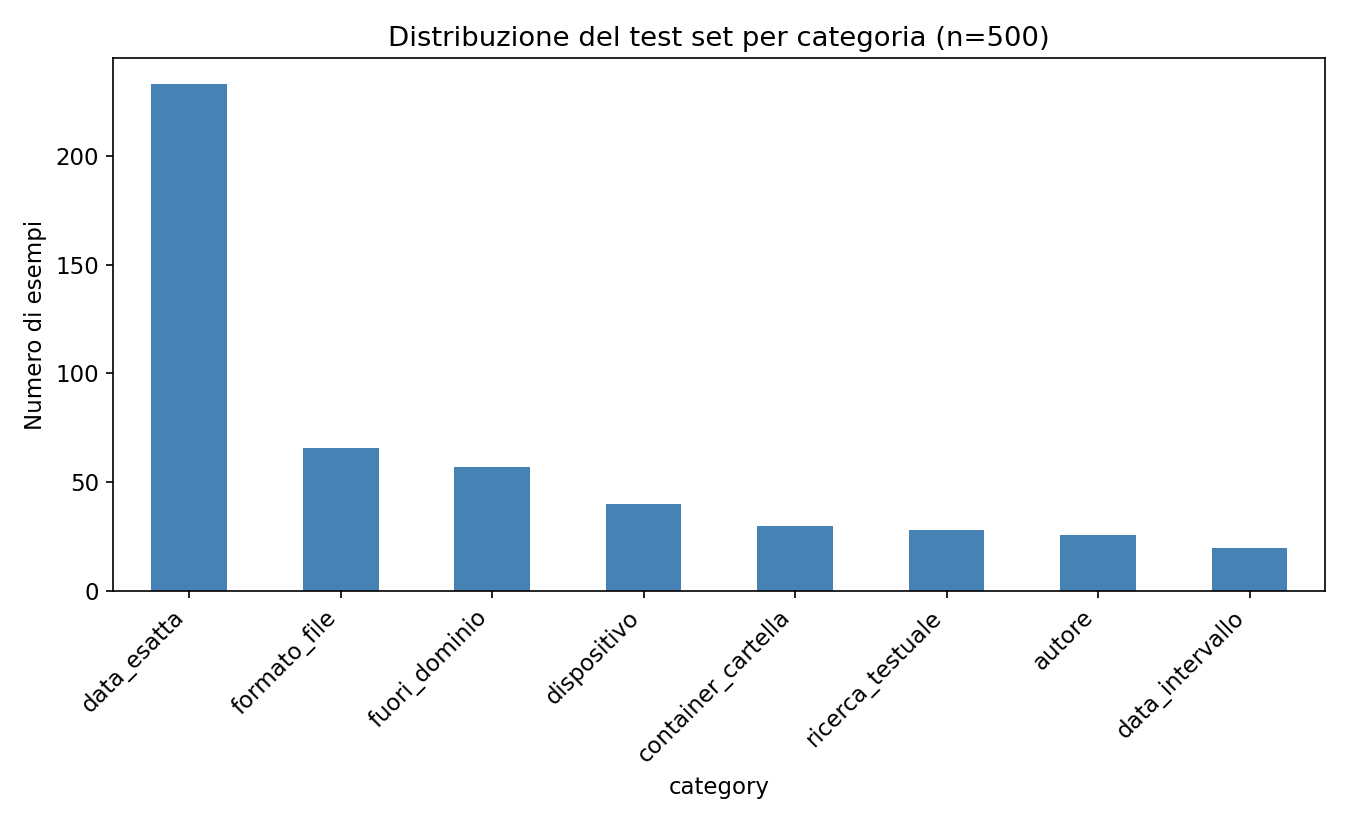
\includegraphics[width=\textwidth]{img/category_distribution.png}
%             % \caption{Distribuzione del test set di valutazione (n=500).}\label{fig:category_distribution}
%         \end{minipage}
%     \end{figure}
% \end{comment}

\newpage
\subsection{Tempo di generazione}\label{subsec:tempo_generazione}

Il tempo di generazione per query, misurato sulla GPU T4 durante la Fase 1, presenta le seguenti statistiche calcolate sull'intero set di 500 esempi:

% --- TABELLA E GRAFICO AFFIANCATI PER RISPARMIARE SPAZIO ---
% \begin{comment}
%     \begin{figure}[htbp]
%         \centering
%         % Minipage di sinistra per la Tabella
%         \begin{minipage}[c]{0.40\textwidth}
%             \centering
%             \begin{tabular}{lr}
%             \toprule
%             Statistica & Valore (s) \\
%             \midrule
%             Media               & 7.45 \\
%             Deviazione standard & 2.51 \\
%             Minimo              & 0.65 \\
%             25° percentile      & 7.64 \\
%             Mediana             & 8.19 \\
%             75° percentile      & 8.59 \\
%             Massimo             & 10.45 \\
%             \bottomrule
%             \end{tabular}
%             % \captionof{table}{Statistiche del tempo di generazione per query (GPU T4).}\label{tab:tempo_generazione}
%         \end{minipage}%
%         \hfill% Spazio flessibile tra tabella e grafico
%         % Minipage di destra per il Grafico
%         \begin{minipage}[c]{0.55\textwidth}
%             \centering
%             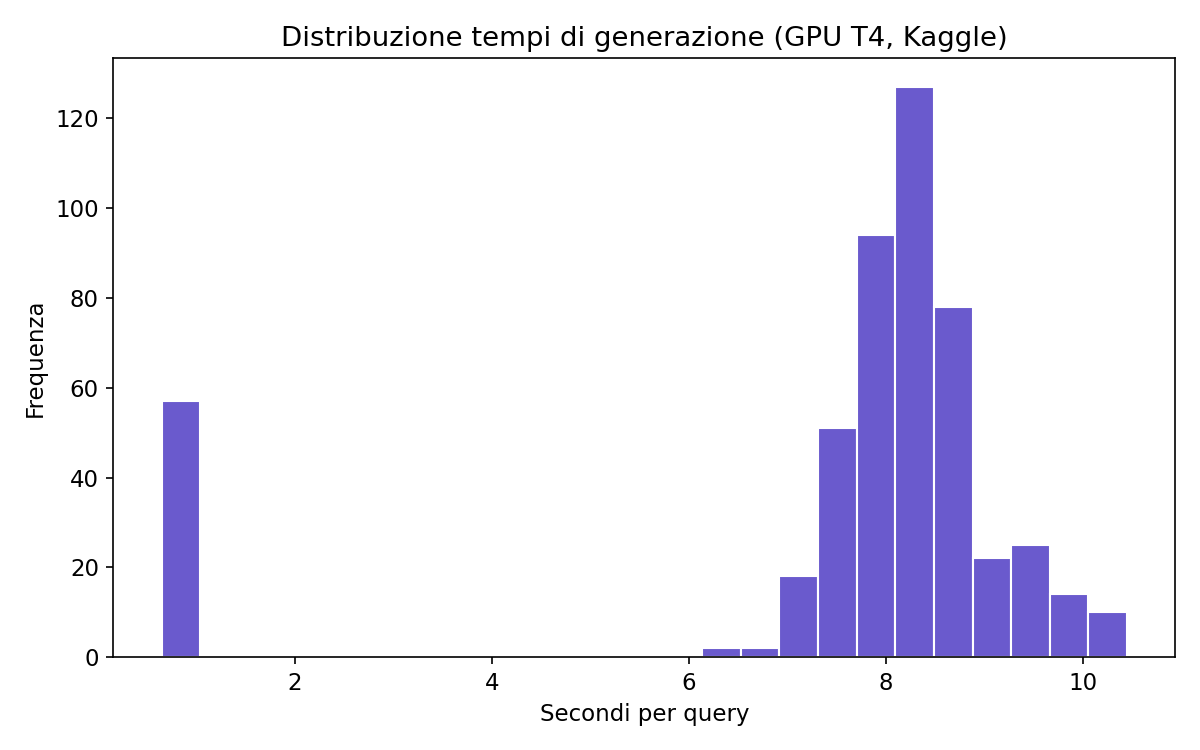
\includegraphics[width=\textwidth]{img/generation_time_hist.png}
%             % \caption{Distribuzione dei tempi di generazione su GPU T4.}\label{fig:generation_time_hist}
%         \end{minipage}
%     \end{figure}
% \end{comment}

\begin{figure}[htbp]
    \centering
    \begin{tabularx}{0.85\textwidth}{X r}
    \toprule
    Statistica & Valore (s) \\
    \midrule
    Media               & 7.45 \\
    Deviazione standard & 2.51 \\
    Minimo              & 0.65 \\
    25° percentile      & 7.64 \\
    Mediana             & 8.19 \\
    75° percentile      & 8.59 \\
    Massimo             & 10.45 \\
    \bottomrule
    \end{tabularx}
    \captionof{table}{Statistiche del tempo di generazione per query (GPU T4).}\label{tab:tempo_generazione}
\end{figure}

\begin{figure}[htbp]
    \centering
    \begin{tikzpicture}
    \begin{axis}[
        ybar interval,
        width=\textwidth,
        height=7cm,
        xlabel={Secondi per query},
        ylabel={Frequenza},
        xmin=0, xmax=11,
        ymin=0,
        minor y tick num=1,
        area style,
        ymajorgrids=true,
        grid style={dashed, gray!30},
        xtick={0,1,2,3,4,5,6,7,8,9,10,11},
        xticklabel style={font=\small},
    ]
    \addplot+[
        hist={bins=22, data min=0, data max=11},
        fill={rgb,255:red,106;green,90;blue,205},
        draw={rgb,255:red,80;green,65;blue,180},
        opacity=0.85,
    ] table [y=time, col sep=space] {../Documenti/generation_times.csv};
    % % Linea verticale per la media
    % \draw[dashed, thick, red!70!black] (axis cs:7.45,0) -- (axis cs:7.45,200)
    %     node[above, font=\footnotesize] {media $= 7{,}45$\,s};
    \end{axis}
    \end{tikzpicture}
    \caption{Distribuzione dei tempi di generazione su GPU T4.}\label{fig:generation_time_hist}
\end{figure}

La distribuzione è concentrata tra i 7 e i 9 secondi per la maggioranza delle query, con una coda di valori bassi (minimo 0.65s) verosimilmente legata a generazioni più brevi, come le risposte \textit{Out-of-Domain}, strutturalmente più corte di una query SPARQL completa.

\subsection{Tasso di esecuzione corretta}\label{subsec:tasso_esecuzione}

Su tutti i 443 esempi non Out-of-Domain del test set, il \textbf{100\% delle query generate è stato eseguito con successo} contro l'endpoint Blazegraph reale, senza errori di sintassi o di esecuzione (\code{execution\_ok = True} per tutte le righe, nessun \code{exec\_error} registrato). Questo dato conferma la validità del system prompt (\cref{subsec:regole}): il modello rispetta rigidamente le regole sintattiche, generando esclusivamente query ben formate.

\subsubsection{Nessun impatto misurato del bug del namespace EXIF}

Il \cref{chap:implementazione} aveva anticipato che l'impatto del namespace EXIF malformato (\cref{subsec:bug_exif_namespace}) sulle metriche di valutazione sarebbe stato verificato in questo capitolo. Il dato è chiaro: \textbf{nessun impatto negativo è stato osservato}. Su 293 dei 443 esempi non Out-of-Domain (categorie \code{data\_esatta}, \code{data\_intervallo} e \code{dispositivo}), la query di riferimento utilizza effettivamente un predicato \code{exif:} nel corpo del \code{WHERE}, non solo nella dichiarazione dei prefissi; tutti e 293 sono stati eseguiti correttamente, con precision e recall pari a 1.000 (\cref{tab:metriche_categoria}).

L'esito attesta il successo della strategia di mitigazione introdotta nel \cref{chap:implementazione}. Avendo allineato il dataset e il backend al namespace malformato di Blazegraph, il sistema non cade nell'errore di usare il prefisso standard (\code{www.w3.org}), che farebbe fallire la query. Se ignorato, il bug avrebbe annullato \textit{precision} e \textit{recall} su quasi due terzi del test set; l'assenza di un calo prestazionale dimostra l'efficacia del workaround, ma il problema originario persiste nei dati di produzione (una criticità architetturale ripresa nel \cref{chap:conclusioni}).

\subsection{Convergenza del training}\label{subsec:convergenza}

Il log di training (\cref{subsec:hyperparams}) mostra una rapida convergenza della loss: da un valore di 0.044 allo step 50 fino a stabilizzarsi attorno a 0.010--0.011 a partire circa dallo step 400, mantenendosi sostanzialmente costante fino al termine dell'addestramento (step 1188, loss finale 0.010).

\begin{figure}[ht]
    \centering
    \begin{tikzpicture}
        \begin{axis}[
            width=\textwidth,
            height=8cm,
            xlabel={Step},
            ylabel={Loss},
            grid=major,
            legend pos=north east,
            xmin=0, xmax=1200,
            ymin=0, ymax=0.05,
            xtick={0, 200, 400, 600, 800, 1000, 1200},
            ytick={0, 0.01, 0.02, 0.03, 0.04, 0.05},
            scaled y ticks=false,
            yticklabel style={
                /pgf/number format/fixed,
                /pgf/number format/precision=2
            },
            tick label style={font=\footnotesize},
            label style={font=\small},
            legend style={font=\footnotesize}
        ]

        \addplot [
            color=blue,
            mark=*,
            mark size=1pt,
        ] table [col sep=comma, x=step, y=loss] {../Documenti/training_log.csv};
        \addlegendentry{Training Loss}

        \addplot [
            color=red,
            mark=square*,
            mark size=1pt,
        ] table [col sep=comma, x=step, y=eval_loss] {../Documenti/training_log.csv};
        \addlegendentry{Validation Loss}

        \end{axis}
    \end{tikzpicture}
    \caption{Andamento della training loss e della validation loss durante il fine-tuning}\label{fig:loss_curve}
\end{figure}

La curva di \textit{validation loss} aderisce a quella di training, escludendo fenomeni di overfitting. Entrambe si stabilizzano intorno allo step 400 su 1188, indicando che il modello avrebbe raggiunto la convergenza anche con un addestramento più breve.

\newpage
% =============================================================================
\section{Efficacia: valutazione qualitativa}\label{sec:efficacia}
% =============================================================================

\subsection{Metriche di retrieval per categoria}\label{subsec:metriche_categoria}

Applicando la metodologia descritta in \cref{subsec:nota_metodologica}, ovvero il confronto sull'insieme completo dei risultati, al netto di \code{ORDER BY}/\code{LIMIT}, le metriche di precision, recall e F1 per categoria sono le seguenti:

\begin{table}[ht]
\centering
\begin{tabular}{lrrrr}
\toprule
Categoria & N & Precision & Recall & F1 \\
\midrule
data\_esatta        & 233 & 1.000 & 1.000 & 1.000 \\
formato\_file       & 66  & 1.000 & 1.000 & 1.000 \\
dispositivo         & 40  & 1.000 & 1.000 & 1.000 \\
container\_cartella & 30  & 1.000 & 1.000 & 1.000 \\
ricerca\_testuale   & 28  & 1.000 & 1.000 & 1.000 \\
autore              & 26  & 1.000 & 1.000 & 1.000 \\
data\_intervallo    & 20  & 1.000 & 1.000 & 1.000 \\
\midrule
\textbf{Media complessiva} & \textbf{443} & \textbf{1.000} & \textbf{1.000} & \textbf{1.000} \\
\bottomrule
\end{tabular}
\caption{Precision, recall e F1 medi per categoria, calcolati sull'insieme completo dei risultati (al netto di \code{ORDER BY}/\code{LIMIT})}\label{tab:metriche_categoria}
\end{table}

Anche il riconoscimento delle richieste Out-of-Domain (\cref{subsec:errori}) raggiunge il 100\% di accuratezza: tutti i 57 esempi fuori dominio nel test set sono stati correttamente classificati come tali dal modello. Allo stesso modo, il \code{limit\_match} (corrispondenza esatta del valore richiesto nella clausola \code{LIMIT}) è verificato nel 100\% dei 443 casi non Out-of-Domain in cui almeno una delle due query include un \code{LIMIT}.

\subsection{Nota critica: interpretazione dei risultati perfetti}\label{subsec:nota_critica}

I risultati perfetti riportati in \cref{tab:metriche_categoria} (punteggio 1.000 su ogni fronte) richiedono un'interpretazione analitica.

Ispezionando il file \code{predictions.json}, emerge che \textbf{le 500 query generate coincidono, carattere per carattere, con le query di riferimento}. Non assistiamo semplicemente a un'equivalenza semantica dei risultati, ma all'esatta riproduzione della stringa SPARQL attesa.

Questo comportamento deriva dalla genesi del test set: essendo prodotto dagli stessi template parametrici (\cref{subsec:dataset_gen}) usati per il training, ne eredita la rigidità strutturale. Le regole del system prompt (\cref{subsec:regole}) restringono drasticamente lo spazio delle query valide, imponendo predicati e costrutti fissi. Di conseguenza, a parità di intento informazionale, la traduzione diventa sostanzialmente deterministica.
\newpage
In altre parole, una corrispondenza esatta al 100\% è coerente con due ipotesi non mutuamente esclusive:

\begin{enumerate}
    \item Il modello ha effettivamente appreso con grande efficacia la mappatura tra intenti linguistici e struttura SPARQL imposta dalle regole, generalizzando correttamente su parametri (anni, dispositivi, nomi di file) anche se non identici a quelli visti in training;
    \item Il test set, essendo generato dallo stesso processo del training set, condivide con esso una distribuzione di superficie sufficientemente vincolata (per via delle 8 regole assolute) da rendere il compito di generazione quasi deterministico, riducendo il valore di questa valutazione come misura di \emph{generalizzazione} a domande realmente nuove e formulate liberamente da un utente umano.
\end{enumerate}

Il codice di inferenza (\code{generate\_predictions.ipynb}) conferma che il test set costituisce una reale partizione \textit{held-out}: l'estrazione è avvenuta in modo deterministico con un rapporto 95\%/5\% e lo stesso seed (\code{3407}) usato per la configurazione del training. Questo esclude \textit{data leakage} o sovrapposizioni (il modello ha elaborato istanze mai viste in fase di addestramento) e avvalora l'ipotesi della generalizzazione strutturale (punto 1), pur confermando che tale generalizzazione avviene strettamente \textit{in-distribution} rispetto ai template.

Ciò non toglie valore al traguardo raggiunto: l'accuratezza del 100\% garantisce un'operatività robusta per l'applicativo. Tuttavia, ne ridimensiona la portata: questa valutazione certifica la disciplina del modello nell'applicare la grammatica del system prompt, ma non la sua capacità di interpretare formulazioni del tutto slegate dai pattern di addestramento. Una prova empirica con ricercatori umani, liberi di porre le proprie domande senza vincoli a priori, rimane un tassello mancante (\cref{chap:conclusioni}).

\subsection{Miglioramento rispetto alle soluzioni precedenti}\label{subsec:miglioramento}

Oltre alle metriche quantitative, l'efficacia si valuta sull'impatto pratico per i ricercatori, risolvendo le barriere esaminate nel \cref{chap:contesto}:

\begin{sloppypar}
\begin{itemize}
    \item \textbf{Funzionalità}: colma l'assenza di un motore di ricerca semantico sul Datavault, affiancando la ricerca per contenuto alla preesistente navigazione per cartelle (\cref{subsec:dharc}).
    \item \textbf{Usabilità}: la barra di ricerca testuale astrae completamente i concetti di triplestore, prefissi RDF e sintassi SPARQL, rendendo accessibile il patrimonio informativo a utenti non tecnici (\cref{subsec:tre_barriere}).
    \item \textbf{Integrazione}: opera come layer aggiuntivo, inserendosi nello stack Fedora/Blazegraph senza richiedere alterazioni dello schema o migrazioni di dati.
    \item \textbf{Manutenzione}: l'architettura modulare (dataset sintetico, prompt, backend isolato) permette di espandere le categorie di query o aggiornare la logica senza impattare il database sottostante.
\end{itemize}
\end{sloppypar}

\subsubsection{Nessun confronto diretto con l'alternativa manuale}

L'analisi appena presentata è prettamente architetturale: manca una validazione empirica. Non abbiamo cronometrato la scrittura manuale delle query SPARQL per i casi d'uso del \cref{chap:prototipo}, né abbiamo sottoposto il sistema a un campione di veri utenti DH.ARC.\@

L'onere sintattico dei casi d'uso (che richiedono l'uso combinato di predicati come \code{exif:make}, \code{exif:dateTime} ed \code{ebucore:hasMimeType} in una singola clausola \code{WHERE}) suggerisce un netto risparmio di tempo e di frustrazione rispetto all'alternativa manuale, in particolare per un'utenza umanistica. Tale beneficio, per ora presunto e supportato dalla teoria del carico cognitivo, dovrà essere quantificato empiricamente. Questo limite metodologico troverà spazio tra gli sviluppi futuri (\cref{chap:conclusioni}).

% =============================================================================
\section{Discussione dei risultati e limiti della valutazione}\label{sec:discussione}
% =============================================================================

I dati raccolti offrono un quadro chiaro sulle prestazioni:

\begin{enumerate}
    \item \textbf{Solidità sintattica}: il vincolo del system prompt (\cref{subsec:regole}) garantisce un tasso di esecuzione privo di errori contro Blazegraph.
    \item \textbf{Tempi di risposta adeguati}: l'elaborazione media di 7.45 secondi su GPU T4 risulta compatibile con un uso esplorativo. Le misurazioni dovranno tuttavia essere estese all'effettivo deployment su CPU (\cref{subsec:tempo_generazione}).
    \item \textbf{Metriche apparentemente perfette}: precisione, recall e F1 a quota 1.000 misurano l'efficacia del modello nel replicare costrutti generati dai template (\cref{subsec:nota_critica}), senza per questo attestare un'analoga robustezza nell'interpretazione di input utente destrutturati.
\end{enumerate}

La natura sintetica del test set rappresenta dunque la principale vulnerabilità dell'analisi. Per saggiare la reale elasticità dell'assistente occorrerà raccogliere una base dati organica, derivante dall'interazione spontanea dei ricercatori del centro (\cref{chap:conclusioni}).